\section{Defining Color Transparency}\label{sec:ct_def}
The phenomenon known as color transparency (CT) was first proposed by
Mueller~\cite{Mueller_1982} and Brodsky~\cite{Brodsky_1982} in 1982.
It is a distinctive feature of QCD's quark degrees of freedom, not arising in a
purely hadronic model.
CT refers to vanishing initial and final state interactions (ISI and FSI)
between hadrons and the surrounding nuclear medium in exclusive processes
at large momentum transfer $Q^2$.
This is in contrast to conventional Glauber theory which assumes strong ISI/FSI
and rescattering.


The existence of CT is a prerequisite for the validity of QCD factorization
theorems~\cite{Brodsky_1994, Collins_1997, Frankfurt_1999, Diehl_1998,
Strikman_2000} which provide access to the Generalized Parton Distributions
(GPDs) that currently provide the most complete picture of the internal
quark-gluon structure of various hadrons~\cite{Ji_1997_Jan, Ji_1997_Jun,
Radyushkin_1996, Radyushkin_1997}.
These theorems assume, at sufficiently large $Q^2$, that deeply inelastic
exclusive processes' amplitudes are separable into two parts: a hard scattering
at the parton level, and a soft part characterized by GPDs.


% insert that nice Feynman diagram
To illustrate the connection between CT and factorization, consider
meson electroproduction.
In the Breit frame, the virtual photon and baryon are both initially at rest.
After the meson absorbs the photon, the meson and baryon both move off in
opposite directions without any further gluon exchange between the two,
provided the meson maintains a small transverse size~\cite{Strikman_2000}.


A QED phenomenon analogous to CT can be seen in the Chudakov effect.
Several experiments have studied the decay $\pi^0 \rightarrow e^+ e^- \gamma$
in photographic emulsions~\cite{Perkins_1955, Fowler_1955, Wolter_1956,
Iwadare_1958, Varfolomeev_1959, Zielinski_1985}.
As an electron-positron pair traveled through the emulsion,
the observed ionization density increased with distance from the decay vertex,
consistent with suppressed interaction between a
small, slowly growing electric dipole and the surrounding medium.
A small $q\bar{q}$ or $qqq$ system or ``point-like configuration'' (PLC) is the
QCD analogue of the QED dipole\footnote{Incidentally, Bjorken used
the reverse of this analogy in 1976 to illustrate why a small
$q\bar{q}$ system shouldn't create jets in hadronic final
states created in electron-positron collisions~\cite{Bjorken_1976}.}.


The existence of CT requires the following criteria:
\begin{itemize}
    \item Scattering takes place by preferentially selecting point-like
          configurations (PLCs) with transverse size much smaller than a
          hadron's ``free'' radius.
    \item Interactions between the PLC and the nuclear medium are reduced.
    \item The PLC's compact size is maintained for a distance comparable to the
          size of the nucleus.
\end{itemize}


\subsection{Squeezing}
The first criterion can be thought of as ``squeezing'' a quark system into a
PLC with transverse size smaller than the radius of the hadron detected in
the final state.


% insert diagram for below?
An intuitive argument from Frankfurt et al.~\cite{Frankfurt_1992} is suggestive
of the possibility of forming a PLC in quasielastic electron scattering from
nuclei.
Suppose a quark in the nucleus, after absorbing a virtual photon, is off-shell
by $\Delta E = Q$.
By the uncertainty principle, its lifetime should be $\tau=1/Q$.
It will decay by emitting a gluon which, if the final state is to include a
proton, must be absorbed by nearby quarks in a radius
$r \approx c \tau \sim 1/Q$.
Thus, for large momentum transfers, the quark system formed in the scattering
process should be quite small.


In 1980, Brodsky and Lepage~\cite{Brodsky_1980, Lepage_1980} showed, using
perturbative QCD (pQCD), that the ``squeezing'' criterion is satisfied for
exclusive processes at large $Q^2$.
In the years following, Isgur and Smith~\cite{Isgur_1984, Isgur_1988,
Isgur_1989} cautioned against the use of pQCD to study exclusive processes,
citing experimental evidence of significant soft contributions to pion and
nucleon form factors.
Experimental support for the dominance of PLCs in these processes will be
discussed in Section~\ref{sec:ct_intermediate_energies}.


\subsection{Reduced Interaction Strength}
The second criterion is a consequence of the PLC's small size;
small configurations of quarks and gluons have small cross sections.
The Low-Nussinov two-gluon exchange
model~\cite{Low_1975, Nussinov_1975, Nussinov_1976} is a simple model of this
phenomenon that treats baryons (mesons) as composed of only the bound states of
valence quarks, $\ket{qqq}$ ($\ket{q\bar{q}}$).
In this model, the hadron-hadron scattering amplitude vanishes as the
transverse size of either of the hadrons vanishes~\cite{Gunion_1977}--
``simply put, color-singlet point particles do not radiate gluons, and cannot
interact via gluon exchange.''
For example, the couplings to a transferred gluon for the constituents in a
small meson's $q\bar{q}$ pair contribute opposite signs.
The same ``color screening'' effect occurs for small $qqq$ configurations.
Interactions with a hadron's $q\bar{q}$ sea components are similarly
suppressed.


Holographic light-front QCD treats hadrons as a superposition of $n$-particle
Fock states $\ket{n}$~\cite{Brodsky_2015}.
In these states, $n$ is constrained such that the difference between the number
of quarks and antiquarks is three for baryons and zero for mesons.
For example, the proton can be written
\begin{align}
    \ket{p} &= \sum_n \qprod{n}{p} \ket{n} \\
            &= \psi_{3q/p}       \ket{uud}
            +  \psi_{3qg/p}       \ket{uudg}
            +  \psi_{4q\bar{q}/p} \ket{uudu\bar{u}}
            +  \psi_{4q\bar{q}/p} \ket{uudd\bar{d}} + \ldots \nonumber
\end{align}
where $\psi_{n/H}$ is the $n$-body light-front wavefunction for a hadron $H$.
A hadron's form factor $F(Q^2)$ can be calculated with these wavefnctions, from
which the transverse size $a_\perp^2(Q^2)$ can be calculated
\begin{equation}
    a_\perp^2(Q^2) = -4\frac{ \frac{d}{dQ^2} F(Q^2) }{ F(Q^2) }
\end{equation}
In light-front holographic QCD, for a hadron of twist\footnote{the number of
constituent quarks of the hadron's valence state}
$\tau$ at large $Q^2$, this expression approaches~\cite{Brodsky_2021}
\begin{equation}
    a_\perp^2(Q^2) = \frac{ 4(\tau-1) }{ Q^2 }
\end{equation}
The value of $Q^2$ required to contract a hadron's valence constituents to a
color-singlet of a given transverse size grows with the number of constituents
as shown in Fig~\ref{fig:brodsky_transverse_size_2021}.

\begin{figure}[!h]
    \centering
    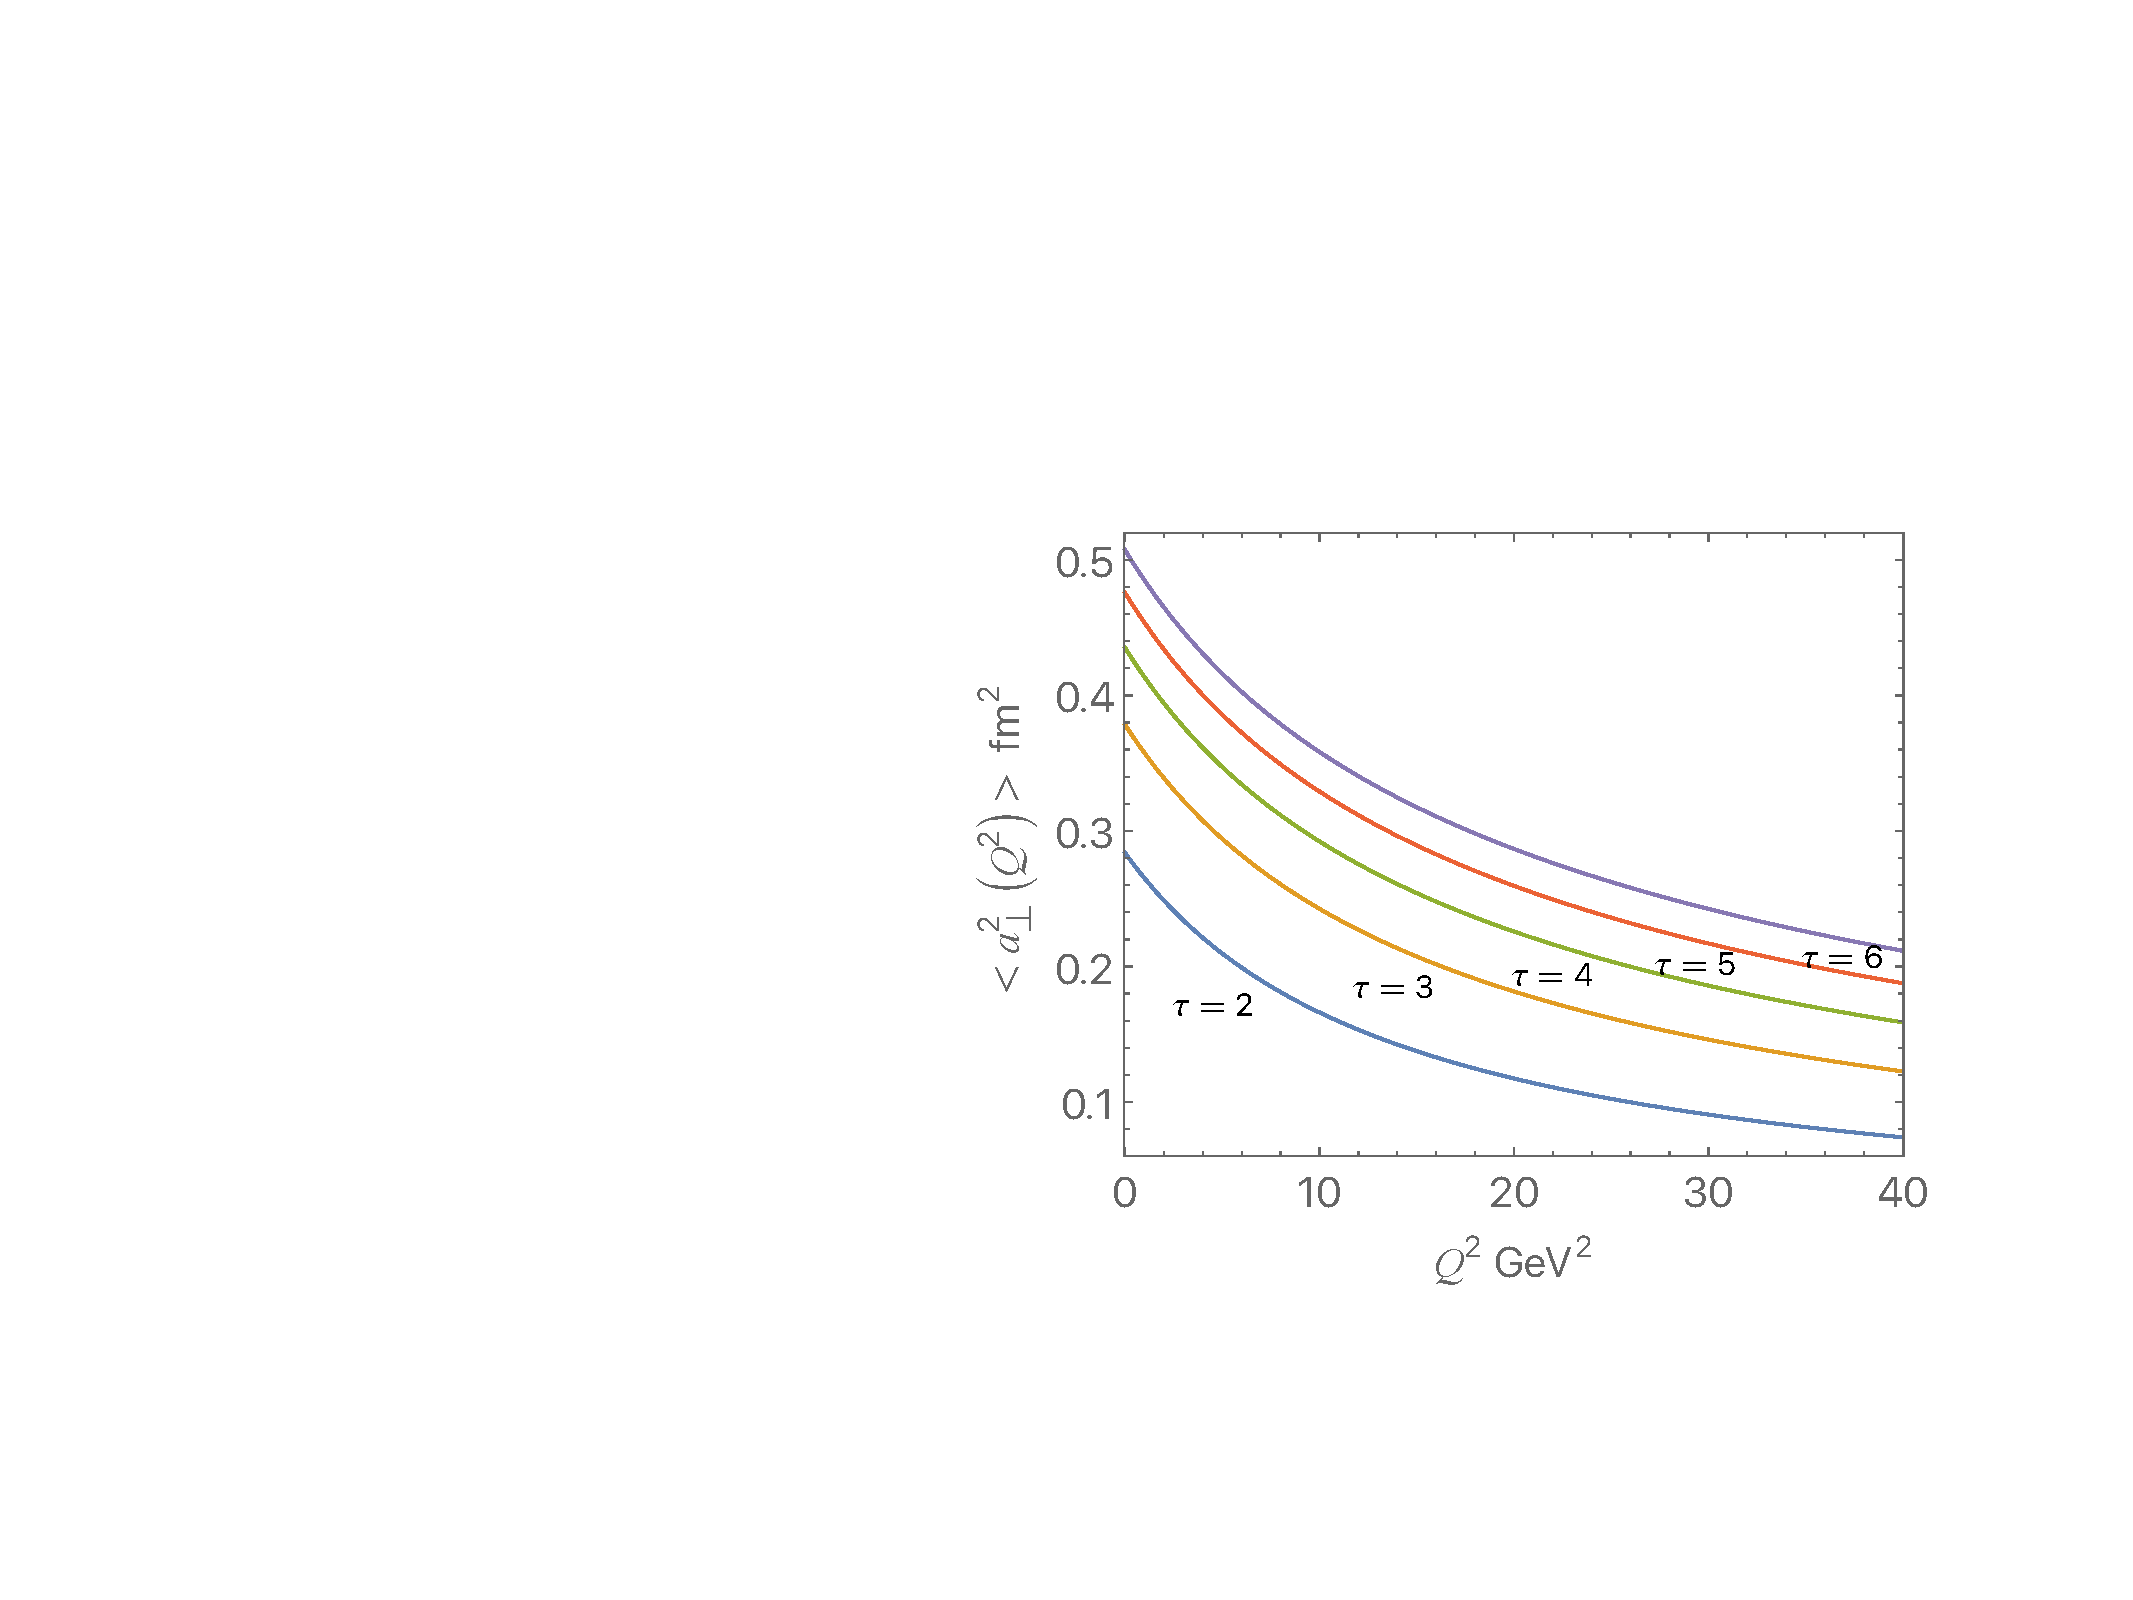
\includegraphics[width=0.8\textwidth]{chap2/brodsky_transverse_size_2021.pdf}
    \caption{
            The transverse size of a hadron with twist $\tau$ as a function of
            momentum transfer $Q^2$, as predicted by light-front holographic
            QCD.
            Figure reproduced from Ref~\cite{Brodsky_2021}.
            }
    \label{fig:brodsky_transverse_size_2021}
\end{figure}




\subsection{Freezing and Expansion}
Suppose a PLC is created in the interior of a nucleus and, in its rest frame,
expands to a configuration with normal size over a time $\tau_0$.
Taking time dilation into account, it expands in a time $\tau=\tau_0E/m$ in the
rest frame of the nucleus over a distance called the coherence length $l_c$.
For large enough energy $E$, $l_c$ is larger than the nuclear diameter and the
PLC can be described as ``frozen'' in its small transverse size as it escapes
the nucleus.
High energy processes where this is indeed the case will be discussed in
Section~\ref{sec:ct_high_energies}.


At intermediate energies however, one must take into account the expansion of
the PLC.
Using the uncertainty principle, the decoherence time can be
estimated, as in Ref~\cite{Farrar_1988}, for an intermediate PLC state with mass
$m_{inter}$ and ``normal'' mass $M_h$:
\begin{align}
    \Delta E &= \sqrt{p_h^2 + m_{inter}^2} - \sqrt{p_h^2 + M_h^2} \\
             &= p_h \left( \sqrt{1+\frac{m_{inter}^2}{p_h^2}} -
                           \sqrt{1+\frac{M_h^2}{p_h^2}} \right) \\
             &\approx p_h \left( \frac{m_{inter}^2}{2p_h^2} - \frac{M_h^2}{2p_h^2} \right) \\
             &= \frac{\Delta M_h^2}{2p_h}
\end{align}
where $\Delta M_h^2 = m_{inter}^2 - M_h^2$.
Then, in natural units, $\Delta E \Delta t = 1$ implies that the coherence
length is
\begin{equation}
    l_c = \frac{2p_h}{\Delta M_h^2}.
\end{equation}
The freezing approximation is valid if $l_c \gg R_A$ where $R_A$ is the radius of
the relevant nucleus.


Ref~\cite{Farrar_1988} also presents an estimate of the effective PLC-nucleon
cross section as a function of propagation distance $z$.
The model assumes that the effective cross section is scaled by the transverse
size of the quark system $x_t$ relative to the average size of the hadron
$\langle x_t \rangle$.
That is
$\sigma^{eff}_{hN} = \left[ x^2_t(z) / \langle x_t \rangle^2 \right] \sigma^{tot}_{hN}$


Let $n$ be the number of partons in the quark system,
$\langle k_t \rangle$ the average transverse momentum of a parton in the
hadron, and $t=-Q^2$ the momentum transfer squared.
Then the transverse area occupied by the quark system is
$\sigma^{tot}_{hN}(n^2 \langle k_t \rangle^2 / t)$ at the point of interaction.
The system expands over the coherence length $l_c$ to its normal hadronic size.


% TODO: change tau to another letter. Confusing because I also use it for lifetime.
% TODO: expand on the models?
% TODO: simplify and just use quantum diffusion?
The effective cross section is then
\begin{equation}
    \sigma_{hN}^{eff} = \sigma_{hN}^{tot}
    \left(
        \left\{\left(\frac{z}{l_c}\right)^{\tau} +
               \frac{\left\langle n^{2} k_{t}^{2}\right\rangle}{t} \left[1-\left(\frac{z}{l_c}\right)^{\tau}\right]
        \right\}
        \theta\left(l_c-z\right) +
        \theta\left(z-l_c\right)
    \right)
\end{equation}
The parameter $\tau$ distinguishes three models:
non-perturbative QCD ($\tau=0$; no reduction in cross section),
pQCD ($\tau=1$; $x_t$ grows like $\sqrt{z}$), and
a naive parton model ($\tau=2$; $x_t$ grows like $z$).


Another approach~\cite{Jennings_1990, Jennings_1991, Jennings_1992}
expands the PLC wave function in terms of hadronic eigenstates
$\ket{\psi_i}$ of the Hamiltonian.
Let $P$ be the PLC's momentum and assume each eigenstate satisfies
$E_i \gg m_i$.
Then
\begin{align}
    \ket{\psi_{PLC}(t)} &= \sum_{i=1}^{\infty} a_i e^{-iE_it}\ket{\psi_i} \\
                        &= e^{-iE_1t} \sum_{i=1}^{\infty} e^{-i\frac{(m_i^2-m_1^2)t}{2P}} \ket{\psi_i}
\end{align}

This suggests that the loss of coherence is due to the relative phase between
hadronic components.
In other words, the coherence length is the length at which coherence between
the lowest and first excited states is lost.


% \subsection{The Significance of Color Transparency}
% CT was originally discussed in the context of pQCD, but has been shown to be
% a general feature of other non-perturbative approaches~\cite{Frankfurt_1992}.


The existence of CT is a prerequisite for the validity of QCD factorization
theorems~\cite{Brodsky_1994, Collins_1997, Frankfurt_1999, Diehl_1998,
Strikman_2000} which provide access to the Generalized Parton Distributions
(GPDs) that currently provide the most complete picture of the internal
quark-gluon structure of various hadrons~\cite{Ji_1997_Jan, Ji_1997_Jun,
Radyushkin_1996, Radyushkin_1997}.
These theorems assume, at sufficiently large $Q^2$, that deeply inelastic
exclusive processes' amplitudes are separable into two parts: a hard scattering
at the parton level, and a soft part characterized by GPDs.

% insert that nice Feynman diagram
To illustrate the connection between CT and factorization, consider
meson electroproduction.
In the Breit frame, the virtual photon and baryon are both initially at rest.
After the meson absorbs the photon, the meson and baryon both move off in
opposite directions without any further gluon exchange between the two,
provided the meson maintains a small transverse size~\cite{Strikman_2000}.


% TODO: Bjorken scaling?
% % Section 4 of this long review
% Relevant longitudinal distance is $y\sim 1 / 2 M_n x$~\cite{Frankfurt_1988}.
% For small $x$, this is larger than the size of the nucleus.
